\begin{figure*}[t]
\centering
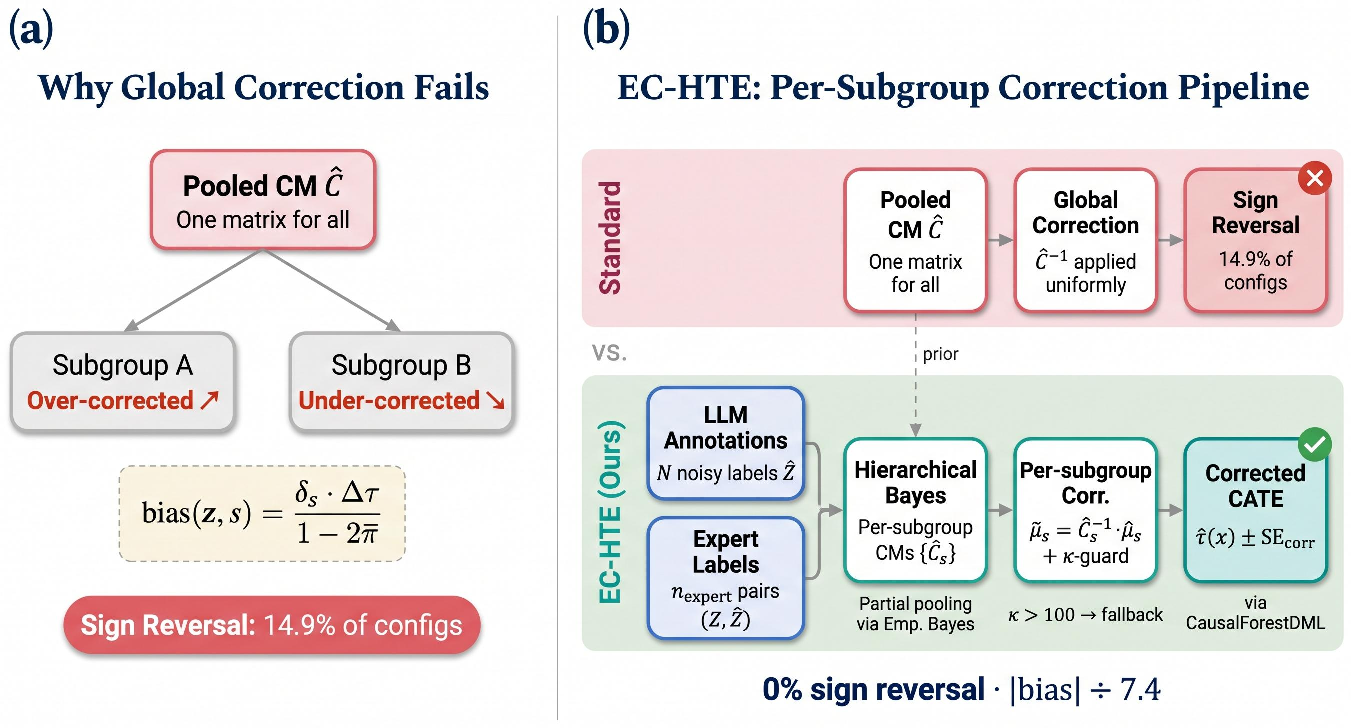
\includegraphics[width=\textwidth]{figures/fig_combined_overview.pdf}
\caption{Overview. (a)~Global correction over/under-corrects subgroups with heterogeneous error rates, introducing bias $\delta_s \cdot \Delta\tau / (1{-}2\bar{\pi})$ (where $\delta_s$ is subgroup error-rate deviation, $\Delta\tau$ is effect heterogeneity, $\bar{\pi}$ is pooled error rate; formally defined in Theorem~\ref{thm:bias_identity}) that reverses conditional average treatment effect (CATE) sign in 14.9\% of configurations. (b)~\textit{Top (rose):} standard pipeline applies a pooled confusion matrix uniformly; \textit{bottom (teal):} EC-HTE estimates per-subgroup matrices via hierarchical Bayes, applies stratified inversion with a condition-number ($\kappa$) guard, and propagates uncertainty.}
\label{fig:method_overview}
\end{figure*}

\section{Introduction}
\label{sec:intro}

Large language models (LLMs) now routinely classify text for computational social science at costs orders of magnitude below manual coding~\cite{gilardi2023chatgpt,tornberg2024chatgpt,ziems2024nlp,tan2024llm}, and a standard safeguard has emerged: validate a sample against expert annotations, estimate a confusion matrix, and apply its inverse to correct the noisy labels.\footnote{Throughout, ``debiasing'' refers to correction of annotation measurement-error bias, not algorithmic fairness debiasing.}
Suppose a researcher uses GPT-4 to classify thousands of posts and then applies this correction to estimate whether a content moderation policy reduces hate speech differently across demographic groups.
The corrected analysis concludes the policy \emph{increases} hate speech among younger users, yet the true effect is protective.
This sign reversal is not an edge case.

The root cause is that LLM error rates are not uniform across subgroups.
\citet{ashwin2025bias} document rates varying by up to $5\times$ across demographic groups; in our pilot, GPT-4.1 error rates vary substantially across text-feature subgroups (error-rate heterogeneity $\Delta\pi = \max_s \pi_s - \min_s \pi_s$; Section~\ref{sec:bias_mechanism}).
When these labels serve as effect modifiers in heterogeneous treatment effect (HTE) analysis, a pooled confusion matrix calibrated for the average error rate over-corrects low-error subgroups and under-corrects high-error ones, distorting conditional average treatment effect (CATE) estimates in opposite directions.

We quantify this effect: global correction reverses the sign of estimated CATE in 14.9\% of configurations ($\tau = +0.03 \to \hat{\tau} = -0.059$; Figure~\ref{fig:sign_reversal}), with the rate increasing as true effects shrink (Figure~\ref{fig:sign_reversal_rate}), and all nine real LLMs tested amplify bias.
To formalize the mechanism, we derive an exact bias identity (Theorem~\ref{thm:bias_identity}) showing that the subgroup-level distortion is proportional to the product of error-rate deviation and effect heterogeneity.
Existing corrections (prediction-powered inference (PPI)~\cite{angelopoulos2023ppi}, design-based supervised learning (DSL)~\cite{egami2023dsl}, prediction-powered conditional inference (PPCI)~\cite{sui2026ppci}, ForestIV~\cite{bu2023forestiv}) assume homogeneous prediction error and thus cannot detect this interaction (Section~\ref{sec:related}).
Guided by the identity, our per-subgroup correction (EC-HTE; Section~\ref{sec:method}) reduces $|\text{bias}|$ by $7.4\times$ under extreme heterogeneity and eliminates sign reversal in the $K{=}2$ setting.

\begin{figure*}[t]
\centering
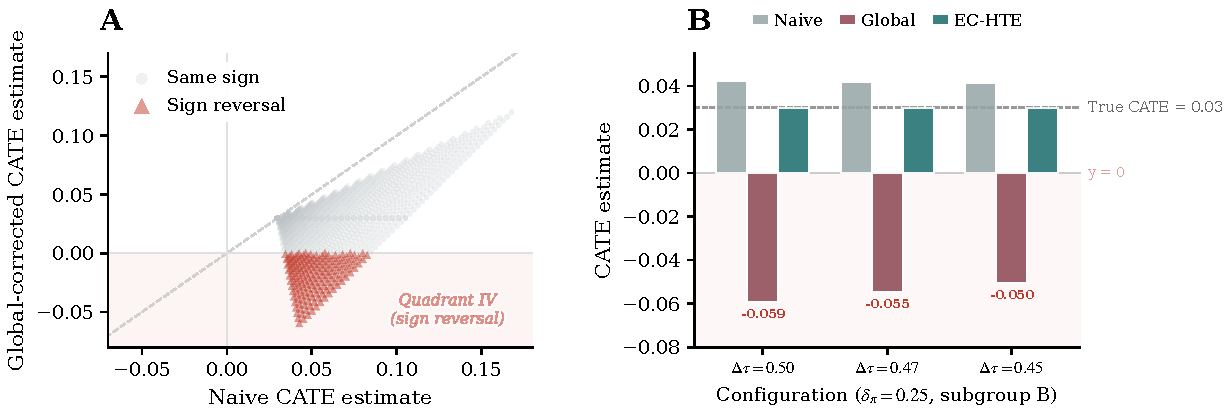
\includegraphics[width=\textwidth]{figures/fig1_sign_reversal.pdf}
\caption{CATE sign reversal under global correction ($K{=}2$, $\tau(0) = 0.03$). (A) Naive vs.\ global-corrected CATE; red triangles mark sign reversals (7.5\% of subgroup estimates). (B) Extreme case: true $\tau = +0.03$, estimated $\hat{\tau} = -0.059$.}
\label{fig:sign_reversal}
\end{figure*}

Our contributions are:
\begin{itemize}
    \item An exact bias identity (Theorem~\ref{thm:bias_identity}): global correction introduces subgroup-level bias $\delta_s \cdot \Delta\tau / (1{-}2\bar{\pi})$, verified at $R^2 \geq 0.97$ across 11 LLM--dataset combinations, with a $\Delta\tau$-free diagnostic (Proposition~\ref{prop:debiasing_hurts}) predicting when correction increases bias from error rates alone.
    \item Empirical operating guidelines: per-subgroup correction outperforms global when $\Delta\pi > 0.15$, $n_{\text{expert}} \geq 250$, and $K \leq 4$.
    \item A concrete instantiation (EC-HTE) using hierarchical Bayesian confusion matrix estimation, verified for difference-in-means (DIM), CausalForestDML, and R-learner, composable with PPCI for joint covariate/outcome error.
\end{itemize}
